\documentclass[dvipdfmx,cjk,xcolor=dvipsnames,envcountsect,notheorems,12pt]{beamer}
% * 16:9 のスライドを作るときは,aspectratio=169 を documentclass のオプションに追加する
% * 印刷用の配布資料を作るときは handout を documentclass のオプションに追加する
% (overlay が全て一つのスライドに出力される)

% \usepackage{pxjahyper}% しおりの文字化け対策 (なくても良い)
\usepackage{amsmath,amssymb,amsfonts,amsthm,ascmac,cases,bm,pifont}
\usepackage{graphicx}
\usepackage{url}

\usepackage{proof}
% \usepackage{tikz}
% \usetikzlibrary{positioning}
\usepackage{algorithm}
\usepackage{algpseudocode}
\usepackage{framed}

\newcommand\intT{\mbox{\texttt{int}}}
\newcommand\boolT{\mbox{\texttt{bool}}}
\newcommand\funT[3]{{#1} \stackrel{#3}{\rightarrow} {#2}}

\newcommand\longer[2]{{#1} \ord {#2}}
\newcommand\uni{\cup}

\newcommand\fun[2]{\lambda{#1}.{#2}}
\newcommand\lam{\lambda}

\newcommand\Resetz{\textbf{reset0}}
\newcommand\Shiftz{\textbf{shift0}}
\newcommand\Throw{\textbf{throw}}
\newcommand\resetz[1]{\Resetz~{#1}}
\newcommand\shiftz[2]{\Shiftz~{#1}\to{#2}}
\newcommand\throw[2]{\Throw~{#1}~{#2}}

\newcommand\Resett{\textbf{reset}}
\newcommand\Shiftt{\textbf{shift}}

\newcommand\cfun[2]{\underline{\lambda}{#1}.{#2}}
\newcommand\clam{\underline{\lambda}}

\newcommand\cResetz{\underline{\textbf{reset0}}}
\newcommand\cShiftz{\underline{\textbf{shift0}}}
\newcommand\cThrow{\underline{\textbf{throw}}}
\newcommand\cresetz[1]{\cResetz~{#1}}
\newcommand\cshiftz[2]{\cShiftz~{#1}\to{#2}}
\newcommand\cthrow[2]{\cThrow~{#1}~{#2}}

\newcommand\cLet{\underline{\textbf{let}}}
\newcommand\cIn{\underline{\textbf{in}}}
\newcommand\clet[3]{\cLet~{#1}={#2}~\cIn~{#3}}
\newcommand\csp[1]{\texttt{\%}{#1}}
\newcommand\code[1]{\texttt{<}{#1}\texttt{>}}

\newcommand\cbra{\texttt{<}}
\newcommand\cket{\texttt{>}}

\newcommand\codeT[2]{\langle{#1}\rangle^{#2}}

\newcommand\codeTs[2]{\langle{#1}\rangle{\textbf{\textasciicircum}{#2}}}
\newcommand\contT[2]{{#1} \Rightarrow {#2}}

\newcommand\ord{\ge}

\newcommand\too{\leadsto^*}
\newcommand\downtoo{\rotatebox{-90}{$\leadsto^*$}}
\newcommand\pink[1]{\textcolor{pink}{#1}}
\newcommand\red[1]{\textcolor{red}{#1}}
\newcommand\green[1]{\textcolor{DarkGreen}{#1}}
\newcommand\magenta[1]{\textcolor{magenta}{#1}}
\newcommand\blue[1]{\textcolor{blue}{#1}}
\newcommand\gray[1]{\textcolor{Gray}{#1}}
\newcommand\lgray[1]{\textcolor{LightGray}{#1}}
\newcommand\black[1]{\textcolor{black}{#1}}
\newcommand\cyan[1]{\textcolor{cyan}{#1}}
\newcommand\pinkbox[1]{\pink{\framebox{#1}}}
\newcommand\redbox[1]{\red{\framebox{#1}}}
\newcommand\greenbox[1]{\green{\framebox{#1}}}
\newcommand\magentabox[1]{\magenta{\framebox{#1}}}
\newcommand\bluebox[1]{\blue{\framebox{#1}}}
\newcommand\blackbox[1]{\black{\framebox{#1}}}
\newcommand\cyanbox[1]{\cyan{\framebox{#1}}}

\newcommand\forin[2]{\textbf{for}~{#1}~\textbf{to}~{#2}~\textbf{in}}
\newcommand\fordo[2]{\textbf{for}~{#1}~\textbf{to}~{#2}~\textbf{do}}
\newcommand\cforin[2]{\underline{\textbf{for}}~{#1}~\underline{\textbf{to}}~{#2}~\underline{\textbf{in}}}
\newcommand\cfordo[2]{\underline{\textbf{for}}~{#1}~\underline{\textbf{to}}~{#2}~\underline{\textbf{do}}}
\newcommand\cfor[1]{\underline{\textbf{for}}~{#1}}
\newcommand\Let{\textbf{let}}
\newcommand\In{\textbf{in}}
\newcommand\cArray[1]{\underline{[{#1}]}}
\newcommand\cArrays[2]{\underline{[{#1}][{#2}]}}
\newcommand\aryset[3]{{#1}[{#2}]\leftarrow {#3}}
% \newcommand\caryset[3]{\underline{\textbf{aryset}}~{#1}~{#2}~{#3}}
\newcommand\caryset[3]{\underline{\textbf{set}}~{#1}~{#2}~{#3}}
\newcommand\set{\underline{\textbf{set}}}

\newcommand\ift[3]{\textbf{if}~{#1}~\textbf{then}~{#2}~\textbf{else}~{#3}}
\newcommand\iif{\textbf{if}}
\newcommand\then{\textbf{then}}
\newcommand\eelse{\textbf{else}}
\newcommand\cif[3]{\underline{\textbf{if}}~\code{{#1}}~\code{{#2}}~\code{{#3}}}
\newcommand\cIf{\underline{\textbf{if}}}

\newcommand\cPlus{\underline{\textbf{+}}}
\newcommand\Plus{\textbf{+}}
\newcommand\cTimes{\underline{\textbf{$\times$}}}
\newcommand\cint{\underline{\textbf{int}}~}
\newcommand\fix{\textbf{fix}}
\newcommand\cfix{\underline{\textbf{fix}}}

\newcommand\lto{\leadsto}
\newcommand\cat{\underline{@}}

\newcommand\ksubst[2]{\{{#1}\Leftarrow{#2}\}}

% スライドのテーマ
\usetheme{sumiilab}
% ベースになる色を指定できる
% \usecolortheme[named=Magenta]{structure}
% 数式の文字が細くて見難い時は serif の代わりに bold にしましょう
% \mathversion{bold}

%% ===============================================
%% スライドの表紙および PDF に表示される情報
%% ===============================================

%% 発表会の名前とか(省略可)
% \session{研究室ゼミ}
%% スライドのタイトル
\title{安全なコード移動が可能な\\コード生成言語の型システムの設計と実装 }

%% 必要ならば,サブタイトルも
% \subtitle{}
%% 発表者のお名前
\author{\underline{{\large 大石純平}} \\  {\scriptsize 指導教員 亀山幸義}}
%% 発表者の所属([] 内は短い名前)
% \institute[東北大学 住井・松田研]{東北大学 工学部 電気情報物理工学科\\住井・松田研究室}% 学部生
\institute[筑波大学 コンピュータサイエンス専攻]{筑波大学 コンピュータサイエンス専攻}% 院生
%% 発表する日
\date{2017/1/27 \\{\tiny 筑波大学修論審査会}}

%% ===============================================
%% 自動挿入される目次ページの設定(削除しても可)
%% ===============================================

% section の先頭に自動挿入される目次ページ(削除すると,表示されなくなる)
\AtBeginSection[]{
  \begin{frame}
    \frametitle{アウトライン}
    \tableofcontents[sectionstyle=show/shaded,subsectionstyle=show/hide/hide]
  \end{frame}}
% subsection の先頭に自動挿入される目次ページ(削除すると,表示されなくなる)
% \AtBeginSubsection[]{
% \begin{frame}
%   \frametitle{アウトライン}
%   \tableofcontents[sectionstyle=show/shaded,subsectionstyle=show/shaded/hide]
% \end{frame}}

%% 現在の section 以外を非表示にする場合は以下のようにする

%% \AtBeginSection[]{
%% \begin{frame}
%%   \frametitle{アウトライン}
%%   \tableofcontents[sectionstyle=show/hide,subsectionstyle=show/show/hide]
%% \end{frame}}
%% \AtBeginSubsection[]{
%% \begin{frame}
%%   \frametitle{アウトライン}
%%   \tableofcontents[sectionstyle=show/hide,subsectionstyle=show/shaded/hide]
%% \end{frame}}

%% ===============================================
%% 定理環境の設定
%% ===============================================

\setbeamertemplate{theorems}[numbered]% 定理環境に番号を付ける
\theoremstyle{definition}
\newtheorem{definition}{定義}
\newtheorem{axiom}{公理}
\newtheorem{theorem}{定理}
\newtheorem{lemma}{補題}
\newtheorem{corollary}{系}
\newtheorem{proposition}{命題}

%% ===============================================
%% ソースコードの設定
%% ===============================================

\usepackage{listings,jlisting}

% \usepackage[scale=0.9]{DejaVuSansMono}

\definecolor{DarkGreen}{rgb}{0,0.5,0}
\definecolor{LightGray}{gray}{0.8}
% プログラミング言語と表示するフォント等の設定
\lstset{
  language={[Objective]Caml},% プログラミング言語
  basicstyle={\ttfamily\small},% ソースコードのテキストのスタイル
  keywordstyle={\bfseries},% 予約語等のキーワードのスタイル
  commentstyle={},% コメントのスタイル
  stringstyle={},% 文字列のスタイル
  frame=trlb,% ソースコードの枠線の設定 (none だと非表示)
  numbers=none,% 行番号の表示 (left だと左に表示)
  numberstyle={},% 行番号のスタイル
  xleftmargin=5pt,% 左余白
  xrightmargin=5pt,% 右余白
  keepspaces=true,% 空白を表示する
  mathescape,% $ で囲った部分を数式として表示する ($ がソースコード中で使えなくなるので注意)
  % 手動強調表示の設定
  moredelim=[is][\itshape]{@/}{/@},
  moredelim=[is][\color{red}]{@r\{}{\}@},
  moredelim=[is][\color{blue}]{@b\{}{\}@},
  moredelim=[is][\color{DarkGreen}]{@g\{}{\}@},
  moredelim=[is][\color{Magenta}]{@m\{}{\}@},
}

%% ===============================================
%% 本文
%% ===============================================
\begin{document}
\frame[plain]{\titlepage}% タイトルページ

\section*{アウトライン}

% 目次を表示させる(section を表示し,subsection は隠す)
\begin{frame}
  \frametitle{アウトライン}
  \tableofcontents[sectionstyle=show,subsectionstyle=hide]
\end{frame}

% 全体 20分-18分
\section{目的}
% コード生成とはプログラムを生成する段階や,生成したプログラムを実行する段階など,複 数のステージを持つプログラミングの手法である.プログラムを計算対象のデータとして扱 うことで,プログラムの効率や,保守性,再利用性 の両立が期待できる.例えば生成元のプ ログラムから,何らかの目的に特化したプログラムを生成を行い,保守や改変をしたい時は, 生成元のプログラムに対して行えばよいので,生成後のコードについては手を加える必要が 無い.そのようなコード生成を効果的に行うためには,言語レベルで,プログラムを生成,実 行などを行う機構を備えることが望ましい.そのような言語をコード生成言語という.

\begin{frame}
  \frametitle{目的}
  % \blue{コード生成の説明と,研究の目的を同時に話す}
  % \vspace{-4zh} %% odd
  \medskip
  \flushleft
  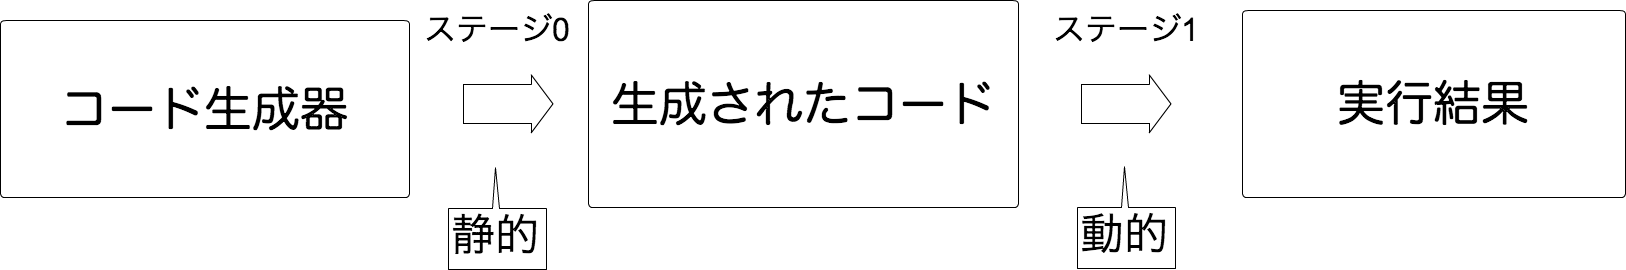
\includegraphics[clip,height=2cm]{./img/prggen.png}

  \begin{itemize}
    % \item コード生成ステージとコード実行ステージ
    % \item 生成前の段階で,生成後のコードの安全性を保証する
  \item コード生成をサポートするプログラム言語\\(=\alert{コード生成言語})
    % \item[◯]<2-> 生成するプログラムだけでなく,生成されたプログラムも型の整合性が静的に (生成前に) 保証される
  \end{itemize}

  \begin{visibleenv}<2>
    \begin{block}{\textbf{表現力}と\textbf{安全性}を兼ね備えたコード生成言語の構築}
      \begin{itemize}
      \item 表現力: 多段階let挿入,メモ化等の技法を表現
      \item 安全性: 生成されるコードの一定の性質を静的に検査
      \end{itemize}
    \end{block}
  \end{visibleenv}

\end{frame}

\begin{frame}
  \frametitle{コード生成前に型付け,生成後のコードの型安全性を保証}
  \begin{onlyenv}<1>
    \center
    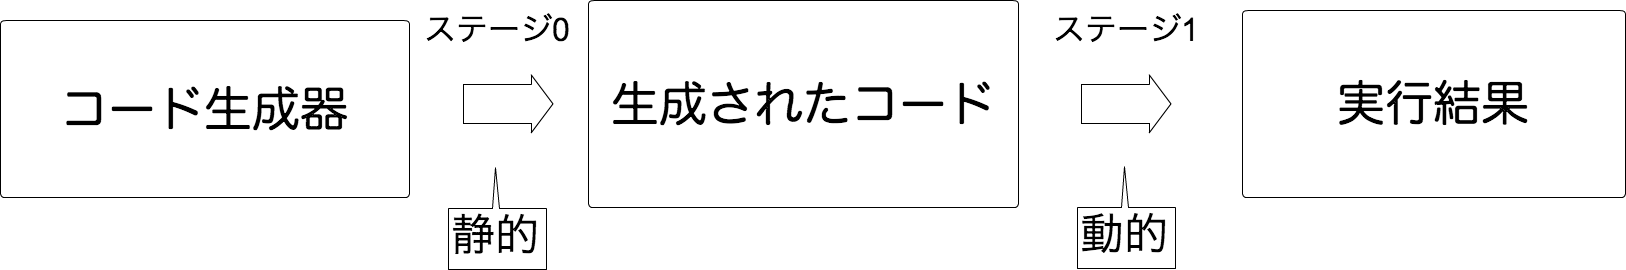
\includegraphics[clip,height=1.9cm]{./img/prggen.png}
  \end{onlyenv}

  \begin{onlyenv}<2>
    \center
    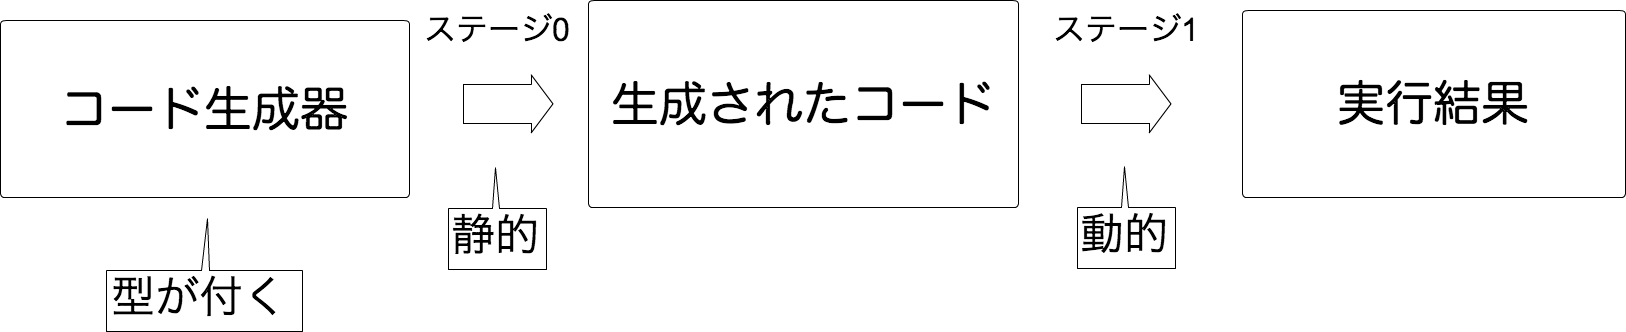
\includegraphics[clip,height=2.4cm]{./img/prggen_type1.png}
  \end{onlyenv}

  \begin{onlyenv}<3>
    \center
    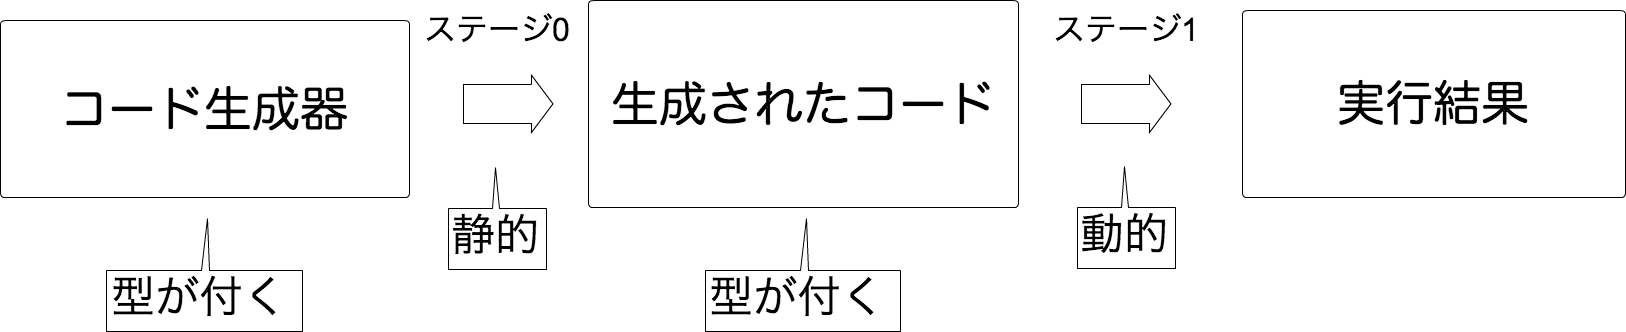
\includegraphics[clip,height=2.4cm]{./img/prggen_type2.png}
  \end{onlyenv}

  \begin{onlyenv}<4>
    \center
    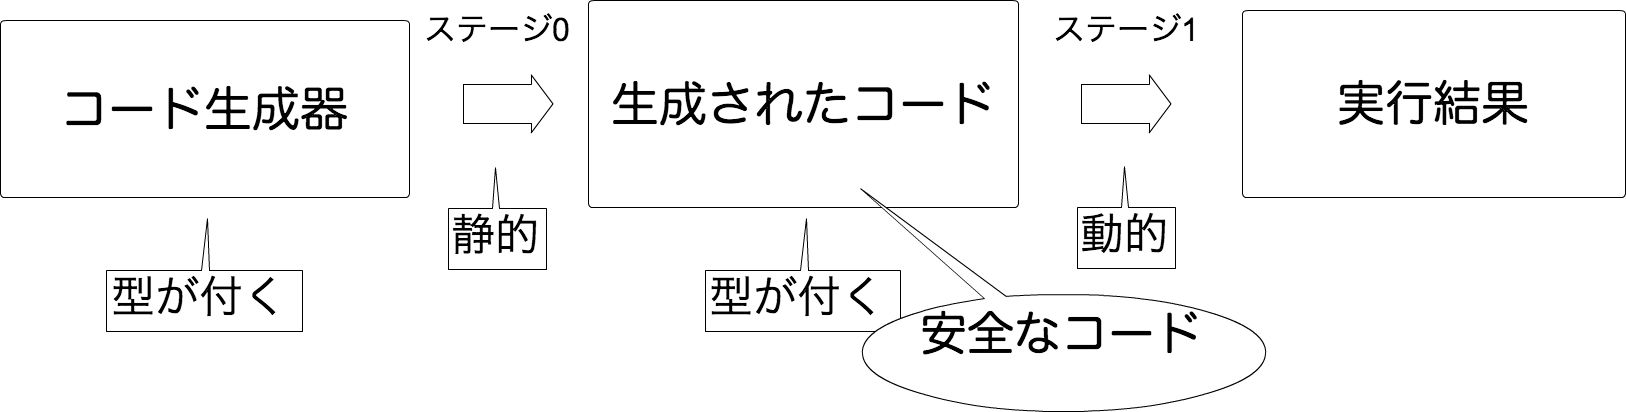
\includegraphics[clip,height=3.0cm]{./img/prggen_type3.png}
  \end{onlyenv}

  \begin{onlyenv}<5->
    \center
    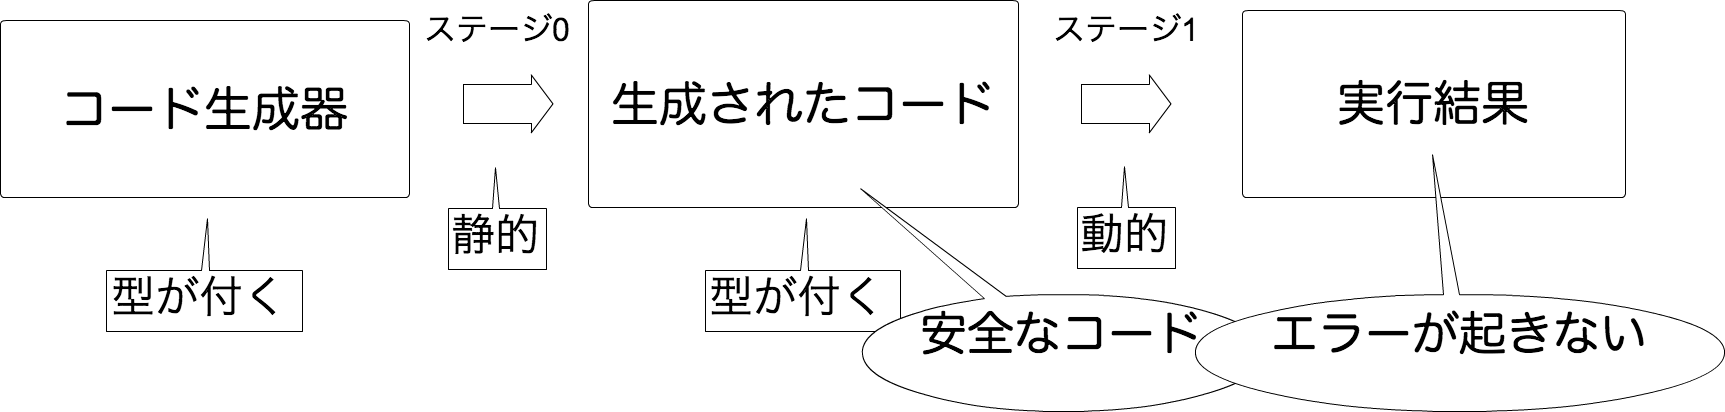
\includegraphics[clip,height=3.0cm]{./img/prggen_type4.png}
  \end{onlyenv}

  \begin{uncoverenv}<6>
    \begin{block}{本研究: 簡潔で強力なコントロールオペレータに基づくコード生成体系の構築}
      \begin{itemize}
      \item コントロールオペレータ shift0/reset0 を利用し,多段階let挿入などのコード生成技法を表現
      \item 型システムを構築して型安全性を保証
      \end{itemize}
    \end{block}
  \end{uncoverenv}

\end{frame}

% \section{研究の目的}
% \begin{frame}
%   \frametitle{研究の目的}

%   \begin{block}{\textbf{表現力}と\textbf{安全性}を兼ね備えたコード生成言語の構築}
%     \begin{itemize}
%     \item 表現力: 多段階let挿入,メモ化等の技法を表現
%     \item 安全性: 生成されるコードの一定の性質を静的に検査
%     \end{itemize}
%   \end{block}

%   \medskip
%   \pause

%   \begin{block}{本研究: 簡潔で強力なコントロールオペレータに基づくコード生成体系の構築}
%     \begin{itemize}
%     \item コントロールオペレータ shift0/reset0 を利用し,let挿入などのコード生成技法を表現
%     \item 型システムを構築して型安全性を保証
%     \end{itemize}
%   \end{block}
% \end{frame}

% \section{研究の内容}

% \begin{frame}
%   \center
%   \huge{表現力を上げ(コードレベルでの多段階let挿入),安全性も保証するためにどうすればよいのか}
% \end{frame}


%%% Local Variables:
%%% mode: latex
%%% TeX-master: "slide_oishi"
%%% End:
 % 目的 2分
\section{準備}

\subsection{コード生成の例}
\begin{frame}
  \frametitle{コード生成言語による記述例}

  \begin{align*}
    \visible<1->{\text{コード生成器}} \visible<1->{&\phantom{\too} \text{生成されるコード}} \\
    \visible<1->{(\cint~ 3)} \visible<1->{&\too \code{3}} \\
    \visible<1->{(\cint~ 3)~ \cPlus~ (\cint~ 5)} \visible<1->{&\too \code{3 + 5}} \\
    \visible<1->{\cfun{x}{~(x~ \cPlus~ (\cint~ 3))}} \visible<1->{&\too \code{\fun{x'}{~(x' + 3)}}} \\
    \visible<1->{\cfordo{x = \cdots}{\cdots}~ \cdots}
    \visible<1->{&\too \code{\fordo{x' = \cdots}{\cdots}~ \cdots}}
  \end{align*}

  % \begin{visibleenv}<2>
  %   \begin{exampleblock}{コードコンビネータ}
  %     \begin{itemize}
  %     \item 下線つきの演算子
  %     \item コードを引数にとり,コードを返す
  %     \end{itemize}
  %   \end{exampleblock}
  % \end{visibleenv}

\end{frame}

\subsection{コード生成器と生成されるコード}

\begin{frame}
  \frametitle{let挿入(コード移動)の実現方法}

  \begin{visibleenv}<1->
    \begin{columns}
      \begin{column}{0.5\textwidth}%% [横幅] 0.2\textwidth = ページ幅の 20 %
        コード生成器
        \begin{align*}
          & ~ \cfordo{x = e1}{e2} \\
          & ~~~ \cfordo{y = e3}{e4} \\
          & ~~~~~~\caryset{\code{a}}{(x,y)}~ ~ \\
          & ~~~~~~~~\magenta{\cLet ~u ~= ~\text{cc} ~\cIn}~~ \text{u}
        \end{align*}
      \end{column}
      $\too$
      \begin{column}{0.5\textwidth}%% [横幅] 0.2\textwidth = ページ幅の 20 %
        生成したいコード
        \begin{align*}
          & \cbra \fordo{x' = e1'}{e2'} \\
          & ~~\magenta{\Let ~u' ~= ~\text{cc}' ~\In} \\
          & ~~~~\fordo{y' = e3'}{e4'} \\
          & ~~~~~~\aryset{a}{x',y'}{u'} \cket
        \end{align*}
      \end{column}
    \end{columns}
  \end{visibleenv}

  \begin{visibleenv}<2>
    \begin{exampleblock}{shift0/reset0の導入}
      \red{shift0/reset0} 等を用いることで,(多段階)let挿入等を行う
    \end{exampleblock}
  \end{visibleenv}
\end{frame}

% \subsection{多段階let 挿入}

% \begin{frame}
%   \frametitle{shift0/reset0 によるlet挿入}
%   \noindent
%   \begin{align*}
%     \uncover<3->{\Resetz ~(E[\Shiftz~ k \to e]) ~\leadsto~ e \ksubst{k}{E}}
%   \end{align*}

%   \noindent

%   %   \begin{align*}
%   %     \text{コード生成器:}~~
%   %     & \uncover<4->{\blue{\Resetz}} ~~\cfordo{x = e1}{e2} \\
%   %     & ~~\uncover<2-3>{\blue{\Resetz}} ~~\cfordo{y = e3}{e4} \\
%   %     & ~~~~\uncover<2->{\blue{\Shiftz}~\blue{k}~\to}~
%   %     \magenta{\cLet~u=t~\cIn} \\
%   %     & ~~~~~~\uncover<2->{(\blue{\Throw~k}}~(\caryset{a}{(x,y)}{u})
%   %     \uncover<2->{)} \\
%   %     &   \uncover<3,5->{\blue{k}}
%   %     \only<3>{\Leftarrow ~~\cfordo{y = e3}{e4}~[\ ]}
%   %     \only<5->{\Leftarrow ~~\cfordo{x = e1}{e2} ~~\cfordo{y = e3}{e4} ~~[\ ]} \\
%   %     \text{生成コード:}~~
%   %     & \uncover<3,5->{\cbra~}
%   %     \only<3>{\fordo{x' = e1'}{e2'}} \only<5->{\magenta{\Let ~u' ~= ~t' ~\In}} \\
%   %     & ~~
%   %     \only<3>{\magenta{\Let ~u' ~= ~t' ~\In}} \only<5->{\fordo{x' = e1'}{e2'}} \\
%   %     & ~~~~\uncover<3,5->{\fordo{y' = e3'}{e4'}} \\
%   %     & ~~~~~~\uncover<3,5->{\aryset{a}{x',y'}{u'} ~\cket}
%   %   \end{align*}

%   \begin{align*}
%     \scriptsize{\text{コード生成器:}}~~
%     & \uncover<2-3>{\blue{\Resetz}} \only<1-2>{~\cfordo{x = e1}{e2}} \uncover<3>{\green{~\cfordo{x = e1}{e2}}}\\
%     & ~~~~~~~~~~~ \only<1-2>{\cfordo{y = e3}{e4}} \uncover<3>{\green{\cfordo{y = e3}{e4}}}\\
%     & ~~~~~~~~~~~~ \only<1-2>{\set~a~(x,y)~} \only<3>{\green{\set~a~(x,y)}~} \only<4->{~~~~~~~~~~~~~~~} \only<1>{cc} \uncover<2-3>{\blue{\Shiftz~ k \to}} \uncover<2->{\magenta{\cLet~u = cc~\cIn}~ \blue{\Throw~ k}~ u \\}
%     %     & ~~~~~~~~~~~~~~~~~~~~~~~~~~~~~~~~\uncover<2->{\magenta{\cLet~u = cc~\cIn}~ \blue{\Throw~ k}~ u} \\
%     & \uncover<3->{\blue{k} \Leftarrow ~~\green{\cfordo{x = e1}{e2}} \\
%     & ~~~~~~~~~~~\green{\cfordo{y = e3}{e4}} \\
%     & ~~~~~~~~~~~~~\green{\caryset{a}{(x,y)}{}} [\ ]} \\
%     \uncover<5->{\scriptsize{\text{生成コード:}}~~}
%     & \uncover<5->{\cbra~}
%     \uncover<5->{\magenta{\Let ~u' ~= ~cc' ~\In}} \\
%     & ~~~~\uncover<5->{\fordo{x' = e1'}{e2'}} \\
%     & ~~~~~~\uncover<5->{\fordo{y' = e3'}{e4'}} \\
%     & ~~~~~~~~\uncover<5->{\aryset{a}{x',y'}{u'} ~\cket}
%   \end{align*}

%   %   \begin{align*}
%   %     \scriptsize{\text{コード生成器:}}~~
%   %     & \uncover<2->{\blue{\Resetz}}~ \only<1-2>{\cfordo{x = e1}{e2}} \only<3>{\green{\cfordo{x = e1}{e2}}}\\
%   %     & ~~~~~~~~~~~\only<1-2>{\cfordo{y = e3}{e4}} \only<3>{\green{\cfordo{y = e3}{e4}}}\\
%   %     & ~~~~~~~~~~~~\only<1-2>{\set~a~(x,y)~} \only<3>{\green{\set~a~(x,y)~}} \only<1>{cc} \only<2>{\blue{\Shiftz~ k \to} \magenta{\cLet~u = cc~\cIn}~ \blue{\Throw~ k}~ u} \only<3->{\magenta{\cLet~u = cc~\cIn}~ \blue{\Throw~ k}~ u}\\
%   %   %     & ~~~~~~~~~~~~~~~~~~~~~~~~~~~~~~~~\uncover<2->{\magenta{\cLet~u = cc~\cIn}~ \blue{\Throw~ k}~ u} \\
%   %     & \uncover<3->{\blue{k} \Leftarrow ~~ \green{\cfordo{x = e1}{e2}} \\
%   %     & ~~~~~~~~~~~\green{\cfordo{y = e3}{e4}} \\
%   %     & ~~~~~~~~~~~~~\green{\caryset{a}{(x,y)}{}} [\ ]} \\
%   %     \uncover<4->{\scriptsize{\text{生成コード:}}~~}
%   %     & \uncover<4->{\cbra~}
%   %     \uncover<4->{\magenta{\Let ~u' ~= ~cc' ~\In}} \\
%   %     & ~~~~\uncover<4->{\fordo{x' = e1'}{e2'}} \\
%   %     & ~~~~~~\uncover<4->{\fordo{y' = e3'}{e4'}} \\
%   %     & ~~~~~~~~\uncover<4->{\aryset{a}{x',y'}{u'} ~\cket}
%   %   \end{align*}
% \end{frame}


% \begin{frame}
%   \frametitle{shift0/reset0 による\alert{多段階}let挿入}
%   \noindent
%   \begin{align*}
%     \Resetz ~(E[\Shiftz~ k \to e]) ~\leadsto~ e \ksubst{k}{E}
%   \end{align*}

%   \noindent
%   %   \begin{align*}
%   %     \text{コード生成器:}~~
%   %     & \red{\Resetz} ~~\cfordo{x = e1}{e2} \\
%   %     & ~~\blue{\Resetz} ~~\cfordo{y = e3}{e4} \\
%   %     & ~~~~\blue{\Shiftz}~\blue{k_2}~\to~
%   %     \red{\Shiftz}~\red{k_1}~\to~
%   %     \magenta{\cLet~u=t~\cIn} \\
%   %     & ~~~~~~\red{\Throw~k_1}~
%   %     (\blue{\Throw~k_2}~(\caryset{a}{(x,y)}{u})) \\
%   %     %     & \red{k_1} \Leftarrow ~~\cfordo{x = e1}{e2}~[\ ] \\
%   %     %     & \blue{k_2} \Leftarrow ~~\cfordo{y = e3}{e3}~[\ ] \\
%   %     \text{生成コード:}~~
%   %     & \cbra~\magenta{\Let ~u' ~= ~t' ~\In} \\
%   %     & ~~\fordo{x' = e1'}{e2'} \\
%   %     & ~~~~\fordo{y' = e3'}{e4'} \\
%   %     & ~~~~~~\aryset{a}{x',y'}{u'} ~\cket
%   %   \end{align*}

%   \begin{align*}
%     \scriptsize{\text{コード生成器:}}~~
%     & \red{\Resetz} ~~\cfordo{x = e1}{e2} \\
%     & ~~\blue{\Resetz} ~~\cfordo{y = e3}{e4} \\
%     & ~~~~ \caryset{a}{(x,y)}{\blue{\Shiftz~ k_1 \to}~ \magenta{\cLet~ u = cc1~ \cIn~} \blue{\Throw~ k_1}~ u;} \\
%     & ~~~~ \set~ b~ (x,y)~ \blue{\Shiftz~ k_1 \to~} \red{\Shiftz~ k_2 \to}~ \\
%     & ~~~~~~~~~~~~~~~~~~~~~~~~ \magenta{\cLet~ w = cc2~ \cIn~} \red{\Throw~ k_2} (\blue{\Throw~ k_1}~ w) \\
%     %     & \red{k_1} \Leftarrow ~~\cfordo{x = e1}{e2}~[\ ] \\
%     %     & \blue{k_2} \Leftarrow ~~\cfordo{y = e3}{e3}~[\ ] \\
%     \uncover<2->{\scriptsize{\text{生成コード:}}~~}
%     & \uncover<2->{\cbra~\magenta{\Let ~w' ~= ~cc2' ~\In}} \\
%     & \uncover<2->{~~~~\fordo{x' = e1'}{e2'}} \\
%     & \uncover<2->{~~~~~~\magenta{\Let ~u' ~= ~cc1' ~\In}} \\
%     & \uncover<2->{~~~~~~~~\fordo{y' = e3'}{e4'}} \\
%     & \uncover<2->{~~~~~~~~\aryset{a}{x',y'}{u'}} \\
%     & \uncover<2->{~~~~~~~~\aryset{b}{x',y'}{w'} ~\cket}
%   \end{align*}
% \end{frame}

%%% Local Variables:
%%% mode: latex
%%% TeX-master: "slide_oishi"
%%% End:
 % 準備 3分 s0/r0 + コード生成 で 多段階let挿入
\section{問題点}

% コントロールオペレータによるコード移動を安全に行いたい
% コントロールオペレータs0/r0によるコード移動
% 安全に

% \begin{frame}
%   \center
%   \huge{問題点}
% \end{frame}

\begin{frame}
  \frametitle{コード生成前後でコードが移動する}
  \begin{visibleenv}<1->
    \begin{columns}
      \begin{column}{0.5\textwidth}%% [横幅] 0.2\textwidth = ページ幅の 20 %
        コード生成器
        \begin{align*}
          & \cfordo{x = e1}{e2} \\
          & ~~\red{\Resetz~} \cfordo{y = e3}{e4} \\
          & ~~~~\red{\Shiftz~} k \to \magenta{\cLet~ u = y ~ \cIn} \\
          & ~~~~~~\red{\Throw~} k~ (\caryset{a}{(x,y)}{u})
        \end{align*}
      \end{column}
      $\too$
      \begin{column}{0.5\textwidth}%% [横幅] 0.2\textwidth = ページ幅の 20 %
        生成されるコード
        \begin{align*}
          & \cbra~ \fordo{x' = e1'}{e2'} \\
          & ~~\magenta{\Let~ u' = y' ~ \In} \\
          & ~~~~\fordo{y' = e3'}{e4'} \\
          & ~~~~~~\aryset{a}{(x',y')}{u'}~ \cket
        \end{align*}
      \end{column}
    \end{columns}
  \end{visibleenv}

  \begin{visibleenv}<2>
    \begin{exampleblock}{Scope Extrusion}
      (コード移動により)意図した束縛から,変数が抜け出てしまうこと
    \end{exampleblock}
  \end{visibleenv}
\end{frame}

% \begin{frame}
%   \frametitle{コード生成前・後でスコープの包含関係が逆転}
%   % sudo らの研究の EC を素朴に適用させると問題があるということ言うスライド
%   % ここに,forループとshift0/reset0 の例を再掲する.
%   % もとのスライドの 24ページの絵をかく.

%   \newcommand\ml{\multicolumn}
%   \begin{columns}
%     \only<1>{コード生成器:}
%     \begin{column}{0.6\textwidth}%% [横幅] 0.2\textwidth = ページ幅の 20 %
%       \center
%       \footnotesize
%       \begin{tabular}{l|l|l|l|l|l|l|l|l|l|l}
%         \cline{2-10}
%         & \ml{9}{|l|}{$\cfordo{x = e1}{e2}$~~~~~~~~~~~~~~~} \\ \cline{3-9}
%         & \footnotesize{\alert{$\mathbf \gamma0$}} & \ml{7}{|l|}{$\Resetz~ \cfordo{y = e3}{e4}$~} & \\ \cline{4-8}
%         & & \footnotesize{\alert{$\mathbf \gamma1$}} & \ml{5}{|l|}{$\Shiftz~ k \to \magenta{\cLet~ u = cc ~ \cIn}$}  & & \\ \cline{5-7}
%         & & & \footnotesize{\alert{$\mathbf \gamma2$}} & \ml{3}{|l|}{$\Throw~ k$}     &   &  &       \\ \cline{6-6}
%         & & & & \footnotesize{\alert{$\mathbf \gamma3$}} & \ml{1}{|l|}{$\caryset{a}{(x,y)}{u}$} & & &  &  \\ \cline{6-6}
%         & & & & \ml{3}{|l|}{\ }  &   &   &           \\ \cline{5-7}
%         & & & \ml{5}{|l|}{\ } &  &               \\ \cline{4-8}
%         & & \ml{7}{|l|}{\ }  & \\ \cline{3-9}
%         & \ml{9}{|l|}{~~~~~~~ } \\ \cline{2-10}
%       \end{tabular}
%     \end{column}

%     \begin{column}{0.5\textwidth}%% [横幅] 0.2\textwidth = ページ幅の 20 %
%       \begin{onlyenv}<2->
%         \flushright
%         \footnotesize
%         \begin{align*}
%           \gamma3 \ord \red{\gamma2} \ord \red{\gamma1} \ord \gamma0 \\
%         \end{align*}
%       \end{onlyenv}

%     \end{column}
%   \end{columns}

%   \bigskip

%   \begin{columns}
%     \only<1>{生成コード:~~}
%     \begin{column}{0.6\textwidth}%% [横幅] 0.2\textwidth = ページ幅の 20 %
%       \footnotesize
%       \begin{tabular}{l|l|l|l|l|l|l|l|l|l|l|l|l|}
%         \cline{2-10}
%         & \ml{9}{|l|}{$\cbra$ $\fordo{x' = e1'}{e2'}$~~~~~~~~~~~~~~~} \\ \cline{3-9}
%         & \footnotesize{\alert{$\mathbf \gamma0$}} & \ml{7}{|l|}{\magenta{$\Let~ u' = cc' ~ \In$}~} & \\ \cline{4-8}
%         & & \footnotesize{\alert{$\mathbf \gamma2$}} & \ml{5}{|l|}{$\fordo{y' = e3'}{e4'}$}  & & \\ \cline{5-7}
%         & & & \footnotesize{\alert{$\mathbf \gamma1$}} & \ml{3}{|l|}{\ }     &   &  &       \\ \cline{6-6}
%         & & & & \footnotesize{\alert{$\mathbf \gamma3$}} & \ml{1}{|l|}{$\aryset{a}{(x',y')}{u'}$ $\cket$} & & &  &  \\ \cline{6-6}
%         & & & & \ml{3}{|l|}{\ }  &   &   &           \\ \cline{5-7}
%         & & & \ml{5}{|l|}{\ } &  &               \\ \cline{4-8}
%         & & \ml{7}{|l|}{\ }  & \\ \cline{3-9}
%         & \ml{9}{|l|}{~~~~~~~ } \\ \cline{2-10}
%       \end{tabular}
%     \end{column}

%     \begin{column}{0.5\textwidth}%% [横幅] 0.2\textwidth = ページ幅の 20 %
%       \begin{onlyenv}<2->
%         \flushright
%         \footnotesize
%         \begin{align*}
%           \gamma3 \ord \red{\gamma1} \ord \red{\gamma2} \ord \gamma0 \\
%         \end{align*}
%       \end{onlyenv}
%     \end{column}
%   \end{columns}
% \end{frame}

%%% Local Variables:
%%% mode: latex
%%% TeX-master: "slide_oishi"
%%% End:
 % 問題 2分
\section{解決策}

\begin{frame}
  \center
  \huge{解決策}
\end{frame}

\begin{frame}
  \frametitle{環境識別子(EC)を利用したスコープ表現\tiny{[Sudo+2014]}}
  % \begin{center}
  %   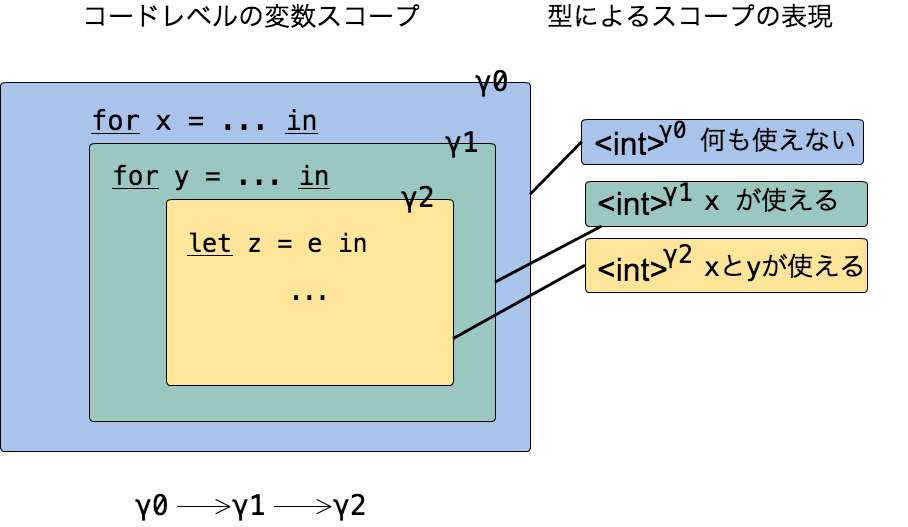
\includegraphics[clip,height=5.7cm]{./img/ec_for.png}
  % \end{center}
  % \begin{flushright}
  %   $\gamma_i ... \text{Refined Environment Classifier}$
  % \end{flushright}

  \newcommand\ml{\multicolumn}
  \center
  {\Large
    \begin{tabular}{l|l|l|l|l|l|}
      \cline{2-6}
      \alert{$\mathbf \gamma0$} & \ml{5}{|l|}{$\cfordo{x = e1}{e2}~~~~~~~~~~~~~~~$} \\ \cline{3-5}
                                & \alert{$\mathbf \gamma1$} & \ml{3}{|l|}{$\cfordo{y = e3}{e4}$} & \\ \cline{4-4}
                                &           & \alert{$\mathbf \gamma2$} & \ml{1}{|l|}{$\caryset{a}{(x,y)} cc$} & ~~ & \\ \cline{4-4}
                                &           & \ml{3}{|l|}{\ }    &               \\ \cline{3-5}
                                & \ml{5}{|l|}{~~~~~~~~~~~~~~~~~~ } \\ \cline{2-6}
    \end{tabular}
  }

  \begin{center}
    \begin{tabular}{c|c}
      スコープ & 使えるコード変数 \\ \hline
      \red{$\gamma0$} & なし \\ \hline
      \red{$\gamma1$} & $x$ \\ \hline
      \red{$\gamma2$} & $x, y$
    \end{tabular}\qquad
  \end{center}

  \red{$\gamma2$} $\ord$ \red{$\gamma1$} $\ord$ \red{$\gamma0$}
\end{frame}

% \begin{frame}
%   \frametitle{環境識別子(EC)を利用したスコープ表現\tiny{[Sudo+2014]}}
%   % 大なり記号はスコープの大きさを表しているのではなく,使える自由変数の集合の大きさを表している
%   型システムでコード変数のスコープを表現:

%   \center
%   \begin{align*}
%     & \Gamma = \gamma2 \ord \gamma1,~
%       x : \codeTs{\textbf{int}}{\gamma1},~
%       y : \codeTs{\textbf{int}}{\gamma2}
%   \end{align*}

%   \begin{tabular}{c|c}
%     $\gamma1$ & $\gamma2$ \\ \hline \hline
%     \uncover<1->{$\Gamma ~\vdash~ x : \codeTs{\textbf{int}}{\gamma1}~~ \alert{\text{OK}}$} & \uncover<1->{$\Gamma ~\vdash~ x : \codeTs{\textbf{int}}{\gamma2}~~ \alert{\text{OK}}$} \\ \hline

%     \uncover<1->{$\Gamma ~\vdash~ y : \codeTs{\textbf{int}}{\gamma1}~~ \alert{\text{NG}}$} & \uncover<1->{$\Gamma ~\vdash~ y : \codeTs{\textbf{int}}{\gamma2}~~ \alert{\text{OK}}$} \\ \hline

%     \uncover<1->{$\Gamma ~\vdash~ x\cPlus y : \codeTs{\textbf{int}}{\gamma1}~~  \alert{\text{NG}}$} & \uncover<1->{$\Gamma ~\vdash~ x\cPlus y : \codeTs{\textbf{int}}{\gamma2}~~  \alert{\text{OK}}$}
%   \end{tabular}

%   \bigskip

%   \begin{uncoverenv}<2->
%     コードレベルのラムダ抽象の型付け規則で固有変数条件を利用:

%     \[
%       \infer[(\gamma_2~\text{is eigen var})]
%       {\Gamma \vdash \cfun{x}{e} : \codeTs{t_1\to t_2}{\gamma_1} }
%       {\Gamma,~\gamma_2 \ord \gamma_1,~x:\codeTs{t_1}{\gamma_2} \vdash
%         e : \codeTs{t_2}{\gamma_2}}
%     \]
%   \end{uncoverenv}
% \end{frame}

\begin{frame}
  \frametitle{環境識別子(EC)を利用したスコープ表現}

  先行研究:
  \begin{itemize}
  \item 局所的なスコープをもつ破壊的変数をもつコード生成の体系に対する(型安全な)型システムの構築
    [Sudo,Kiselyov,Kameyama 2014]
  \item グローバルなスコープをもつ破壊的変数への拡張
    [Kiselyov,Kameyama,Sudo 2016]
  \item[◯] コントロールオペレータには非対応
  \end{itemize}

  \medskip
  \begin{uncoverenv}<2->
    \begin{exampleblock}{問題点:}
      shift0/reset0 などのコントロールオペレータは,スコープの包含関係を逆転させてしまう.
    \end{exampleblock}
  \end{uncoverenv}
\end{frame}


% \begin{frame}
%   \frametitle{本研究の解決策}
%   \flushleft
%   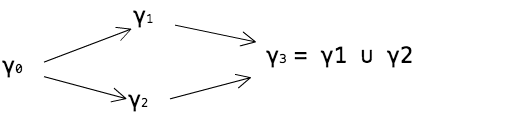
\includegraphics[clip,height=3cm]{./img/ecgraph.png}
%   \begin{itemize}
%   \item<2-> $\gamma1$ のコード変数は $\gamma2$ では使ってはいけない
%   \item<2-> $\gamma2$ のコード変数は $\gamma1$ では使ってはいけない
%   \item<3->[$\Rightarrow$] \red{$\gamma1$ と $\gamma2$ の間に順序を付けない}
%   \end{itemize}

%   \begin{itemize}
%   \item<4-> $\gamma1, \gamma2$ のコード変数は $\gamma3$ で使ってよい
%   \item<5->[$\Rightarrow$] \red{Sudoらの体系に $\cup$ (ユニオン) を追加} % ジョイン
%   \end{itemize}
% \end{frame}

\begin{frame}[fragile]
  \frametitle{コード生成+shift0/reset0 の型システム\small{ (の一部)}}
  reset0:
  \[
    \infer{\Gamma \vdash \resetz{e} : \codeTs{t}{\gamma} ~ \lgray{;~ \sigma}}
    {\Gamma \vdash e : \codeTs{t}{\gamma} ~\lgray{;~ \codeTs{t}{\gamma}, \sigma}}
  \]

  shift0:
  \[
    \infer{\Gamma \vdash \shiftz{k}{e} : \codeTs{t1}{\red{\gamma1}} ~\lgray{;~ \codeTs{t0}{\gamma0},\sigma}}
    {\Gamma,~k:\contT{\codeTs{t1}{\gamma1}}{\codeTs{t0}{\gamma0}}
      \vdash e : \codeTs{t0}{\red{\gamma0}} ~\lgray{;~ \sigma}
      & \Gamma \models \gamma1 \ord \gamma0
    }
  \]

  throw:
  \[
    \infer
    {\Gamma,~k:\contT{\codeTs{t1}{\gamma1}}{\codeTs{t0}{\gamma0}}
      \vdash \throw{k}{v} : \codeTs{t0}{\gamma2} ~\lgray{;~ \sigma}}
    {\Gamma
      \vdash v : \codeTs{t1}{\red{\gamma1 \cup \gamma2}} ~\lgray{;~ \sigma}
      & \Gamma \models \gamma2 \ord \gamma0
    }
  \]
\end{frame}

\subsection{型付けの例}

\newcommand\boxterm{\framebox{
    \only<1>{\phantom{a}}
    \only<2>{\green{$\cint{3}$}}
    \only<3>{\red{$x$}}
  }}

\begin{frame}
  \frametitle{型付けの例(1)}


  {\footnotesize
    \begin{align*}
      e = \Resetz~ \redbox{\cfordo{x = e1}{e2}~ \bluebox{\Shiftz~ k~ →~ \magentabox{\cLet~u=\green{\boxterm}~\cIn~ \cyanbox{\Throw~k~\blackbox{u}}}}} % \to や \rightarrow を \framebox で囲むとなぜかエラーが出る.バグっぽい
    \end{align*}
  }

  \[
    \infer{\vdash e : \codeTs{t}{\gamma0};~\epsilon}
    {\infer[(\gamma1^*)]{\vdash \cfor{x=...} :
        \codeTs{t}{\gamma0};~\codeTs{t}{\gamma0}}
      {\infer{\gamma1 \ord \gamma0,~x:\codeTs{t}{\gamma1}
          \vdash \Shiftz~k~\to~... :
          \codeTs{t}{\gamma1};~\codeTs{t}{\gamma0}}
        {\infer[(\gamma2^*)]{\Gamma a \vdash \cLet~u=...:\codeTs{t}{\gamma0};~\epsilon}
          {\infer{\Gamma b \vdash
              \Throw~k~u:\codeTs{t}{\gamma2};~\epsilon }
            {\infer{\Gamma b \vdash
                u:\codeTs{t}{\gamma1 \cup \gamma2};~ \sigma}
              {}
            }
            &\infer*{\Gamma a \vdash
              \green{\boxterm}:\codeTs{t}{\red{\gamma0}};~\epsilon}
            {}
          }
        }
      }
    }
  \]

  % $[(\gamma1^*)]$ は eigen variable (固有変数)

  {\footnotesize
    \begin{align*}
      \Gamma a &= \blue{\gamma1} \ord \red{\gamma0},~x:\codeTs{t}{\blue{\gamma1}},
                 ~k: \contT{\codeTs{t}{\gamma1}}{\codeTs{t}{\gamma0}} \\
      \Gamma b &= \Gamma a,~\gamma2 \ord \gamma0,~u:\codeTs{t}{\gamma2}
    \end{align*}
  }

\end{frame}

\begin{frame}
  \frametitle{型付けの例(2)}
  % ここでは型付けが複雑になるということを言うにとどめておく

  \newcommand\gammaa{\gamma1 \ord \gamma0,~x:\codeTs{t}{\gamma1}}
  \newcommand\gammab{\Gamma a,\gamma2 \ord \gamma1,~y:\codeTs{t}{\gamma2}}
  \newcommand\gammac{\Gamma b,\blue{k_2}:\contT{\codeTs{t}{\gamma2}}{\codeTs{t}{\gamma1}}}
  \newcommand\gammad{\Gamma c,\red{k_1}:\contT{\codeTs{t}{\gamma1}}{\codeTs{t}{\gamma0}}}
  \newcommand\gammae{\Gamma d,\gamma3 \ord \gamma0,\magenta{u}:\codeTs{t}{\gamma3}}

  \newcommand\boxterms{\framebox{
      \only<2>{\red{$x$}}
      \only<3>{\red{$y$}}
      \phantom{a}
    }}

  \vspace{-1zh} % odd

  \footnotesize
  \begin{align*}
    e'= & \red{\Resetz}~(\cfordo{x = e1}{e2}~\blue{\Resetz} ~(\cfordo{y = e3}{e4} \\
    % & \blue{\Shiftz}~\blue{k_2}\to~ \red{\Shiftz}~\red{k_1}\to~\magenta{\cLet~u=\green{\framebox{\phantom{x}}}~\cIn}
      & \blue{\Shiftz}~\blue{k_2}\to~ \red{\Shiftz}~\red{k_1}\to~\magenta{\cLet~u=\green{\boxterms}~\cIn}
        ~\red{\Throw~k_1}~(\blue{\Throw~k_2}~e5)))
  \end{align*}

  \vspace{-2zh} % odd

  \[
    \infer{\vdash e'=\red{\Resetz}\cdots : \codeTs{t}{\gamma0};~~~\epsilon}
    {\infer[(\gamma1^*)]
      {\vdash \cfor{x=...} : \codeTs{t}{\gamma0};~~~\codeTs{t}{\gamma0}}
      {\infer{\Gamma a=\gammaa\vdash \blue{\Resetz}\cdots : \codeTs{t}{\gamma1};~~~\codeTs{t}{\gamma0}}
        {\infer[(\gamma2^*)]
          {\Gamma a\vdash \cfor{y=...}: \codeTs{t}{\gamma1};~~~\codeTs{t}{\gamma1},\codeTs{t}{\gamma0}}
          {\infer{\Gamma b=\gammab\vdash \blue{\Shiftz~k_2}... :\codeTs{t}{\gamma2}
              ;~~~\codeTs{t}{\gamma1},\codeTs{t}{\gamma0}}
            {\infer{\Gamma c=\gammac\vdash \red{\Shiftz~k_1}... :\codeTs{t}{\gamma1}
                ;~~~\codeTs{t}{\gamma0}}
              {\infer[(\gamma3^*)]
                {\Gamma d=\gammad\vdash \magenta{\cLet~u=...} : \codeTs{t}{\gamma0};~\epsilon}
                {\infer
                  {\Gamma e=\gammae\vdash \red{\Throw~k_1}~... : \codeTs{t}{\gamma3};~\epsilon}
                  {\infer{\Gamma e\vdash \blue{\Throw~k_2}~e5 :
                      \codeTs{t}{\gamma1\cup\gamma3};~~\epsilon}
                    {\infer*{\Gamma e\vdash e5:
                        \codeTs{t}{\gamma2\cup\gamma1\cup\gamma3};~~~\epsilon}
                      {}
                    }
                  }
                  % &\infer*{\Gamma d\vdash \green{\framebox{\phantom{x}}}:\codeTs{t}{\gamma0};\epsilon}{}
                  &\infer*{\Gamma d\vdash \green{\boxterms}:\codeTs{t}{\gamma0};\epsilon}{}
                }
              }
            }
          }
        }
      }
    }
  \]

  {\footnotesize
    \begin{align*}
      \Gamma d &= \cdots,~ x:\codeTs{t}{\red{\gamma1}},~ y:\codeTs{t}{\red{\gamma2}},~ \gamma1 \ord \gamma0,~ \gamma2 \ord \gamma1,~ \cdots
    \end{align*}
  }

\end{frame}

%%% Local Variables:
%%% mode: latex
%%% TeX-master: "slide_oishi"
%%% End:
 %  解決方法 4分 型システム
\begin{frame}
  \center
  \huge{型推論アルゴリズム}
\end{frame}

\begin{frame}
  \frametitle{型推論アルゴリズム}

  $\Gamma,~ L,~ \sigma,~ t,~ e$ が与えられたとき,$\Theta(\Gamma \vdash^{L} e : t ;~\sigma)$ が成立するような代入$\Theta$があるかどうか判定する

  \begin{exampleblock}{制約生成}
    与えられた項に対して,型,EC,エフェクトに関する制約を返す
  \end{exampleblock}
  \begin{exampleblock}{制約解消}
    その得られた制約を解消し,その制約を満たす代入$\Theta$またはfailを返す
  \end{exampleblock}
\end{frame}

% \begin{frame}
%   \frametitle{型推論アルゴリズム}

% \end{frame}

\begin{frame}
  \frametitle{制約生成}
  \begin{exampleblock}{制約生成用の型システム$T_2$}
    \small
    $T_1$
    \vspace{-0.5zh}
    \[
      \infer[]
      {\Gamma \vdash u~ \cPlus~ w: \codeT{\intT}{\gamma}; \sigma}
      {\Gamma \vdash u: \codeT{\intT}{\gamma}; \sigma & \Gamma \vdash w: \codeT{\intT}{\gamma}; \sigma}
      +
      \quad
      \infer
      {\Gamma \vdash e : \codeT{t}{\gamma_2} ; \sigma}
      {\Gamma \vdash e : \codeT{t}{\gamma_1} ; \sigma
        & \Gamma \models \gamma_2 \ord \gamma_1
      }
    \]
    \vspace{-2zh}
    \begin{visibleenv}<2->
      $T_2$\\
      \[
        \infer[Constr;~ \Gamma \models \longer{t}{\codeT{\intT}{\gamma}}]
        {\Gamma \vdash u~ \cPlus~ w: t; \sigma}
        {\Gamma \vdash u: \codeT{\intT}{\gamma}; \sigma & \Gamma \vdash w: \codeT{\intT}{\gamma}; \sigma}
      \]
    \end{visibleenv}
    \vspace{-2zh}
    \begin{itemize}
    \item 下から上に一意的に適用
    \item 規則適用時に制約を生成
    \end{itemize}
    % subsumption 規則をあらゆる規則に付加させて型推論用(制約を生成する)の型システムを作成.
    % 型付け規則を一意に適用できるようにした
  \end{exampleblock}
  \begin{exampleblock}{型に関する順序 $\longer{t_1}{t_2}$}
    % 制約生成時において,コード型か普通の型か判断することができないため
    % その2つを同時に表す$\longer{}{}$ を導入した
    コード型か普通の型か判断できないため,型に関する順序$\ord$の導入を行った
  \end{exampleblock}
  % こういう制約が出てくる
\end{frame}

\begin{frame}
  \frametitle{制約解消}

  % 生成された制約 $\Delta \models C$

  % 仮定 $\Delta$
  % \begin{align*}
  %   &\text{ECに対する順序} & \quad d \ord \gamma \\
  % \end{align*}
  制約 $C$
  \begin{align*}
    &\text{型} & t0 = t1 & \quad t0 \ord t1 \\
    &\text{EC} & \gamma0 = \gamma1 & \quad \only<2->{\red{\gamma0 \ord \gamma1}}\only<1>{\gamma0 \ord \gamma1} \\
    &\text{エフェクト (型の列)} & \sigma0 = \sigma1
  \end{align*}

  \begin{exampleblock}{制約に対する解の存在判定}
    型,EC,エフェクトに対する単一化等をおこなう \\ % 単一化については質問が出そうなのでappendixを作成する
  \end{exampleblock}
  \visible<2->{ここでは,ECの不等式制約の解消について説明をする}
  % 先の制約を解消して,型を決定する
\end{frame}

% \begin{frame}
%   \frametitle{制約解消:ECの不等式制約の解消}
%   この時点で残る制約 $\Delta \models C$
%   \begin{align*}
%     &\text{仮定 $\Delta$} & \quad d \ord e \text{の有限集合 ($d$はEC定数)}\\
%     &\text{制約 $C$} & \quad e1 \ord e2 \text{の有限集合}\\
%     &\text{$e,e1,e2,...$ ECを表す式} & \quad e ::= d \mid x \mid e \uni e\\
%   \end{align*}

%   \vspace{-2.5zh} %% odd

%   \begin{onlyenv}<1>
%     \begin{exampleblock}{制約解消アルゴリズム(の一部)}
%       \begin{description}
%       \item[$d1 \ord d1$] $\Longrightarrow  \text{$\Delta$を使って判定}$
%       \item[$e1 \ord e2 \uni e3$] $\Longrightarrow \text{$e1 \ord e2$ かつ $e1 \ord e3$}$
%       \item[$e1 \uni e2 \ord d$] $\Longrightarrow \text{$e1 \ord d$ または $e2 \ord d$}$
%       \item[$\text{変数 $x$ の除去}$] $[x := d1 \uni d2 \uni y ]$ \mbox{} \\
%         \vspace{-2zh} %% odd
%         \begin{align*}
%           &e1 \ord x & \quad x \ord d1 & \quad \phantom{\Longrightarrow\,\,\,} e1 \ord d1 & \quad e2 \ord d1 \\
%           &e2 \ord x & \quad x \ord d2 & \quad \Longrightarrow e1 \ord d2 & \quad e2 \ord d2 \\
%           &          & \quad x \ord y  & \quad \phantom{\Longrightarrow\,\,\,} e1 \ord y  & \quad e2 \ord y
%         \end{align*}
%       \end{description}
%     \end{exampleblock}
%   \end{onlyenv}

%   % 制約を満たす解が存在するかどうかは判定できる
%   % 解は1つとは限らない

% \end{frame}

\begin{frame}
  \frametitle{制約解消:ECの不等式制約の解消の例}
  \[
    \cfun{x}{(\cint{1}~ \cPlus~ x)} : \visible<-4>{t1} \visible<5->{\codeTs{\funT{\intT}{\intT}{}}{d0}}
  \]

  \begin{align*}
    % & C = \{\invisible<4->{\longer{\gamma2}{\gamma3},~} \longer{d1}{\gamma2},~ \invisible<3->{\longer{\gamma2}{d1},~} \invisible<2->{\longer{\gamma'}{\gamma1}}\} \\
    & C = \{\invisible<4->{\longer{\gamma2}{\gamma3},~} \invisible<3->{\longer{\gamma2}{d1},~} \invisible<2->{\longer{\gamma'}{\gamma1}}\} \\
    & \Theta = \{t1 := \codeTs{\funT{t2}{t3}{}}{\gamma'},~ t2 := \intT,~ t3 := \intT,~ t4 := \intT,~\\
    &\phantom{\Theta =~}\gamma' := d0 \only<2->{,~ \gamma1 := d0} \only<3->{,~ \gamma2 := d1} \only<4->{,~ \gamma3 := d0}\}
  \end{align*}

  \begin{exampleblock}{ECの変数の除去を行う}
    \begin{description}
    \item[$\gamma1$ を選ぶ]<2-> $C$から $\longer{\gamma'}{\gamma1}$ を消去し $\Theta$ に代入$\gamma1 := d0$ を追加
    \item[$\gamma2$ を選ぶ]<3-> $C$から $\longer{\gamma2}{d1}$ を消去し $\Theta$ に代入$\gamma2 := d1$ を追加
    \item[$\gamma3$ を選ぶ]<4-> $C$から $\longer{\gamma2}{\gamma3}$ を消去し $\Theta$ に代入$\gamma3 := d0$ を追加
    \end{description}
  \end{exampleblock}

\end{frame}

\begin{frame}
  \frametitle{研究成果}
  \begin{block}{コード生成 + shift0/reset0 の体系に対する}
    \begin{itemize}
    \item 型システムの設計
    \item 型推論アルゴリズムの開発
    \end{itemize}
  \end{block}
\end{frame}

%%% Local Variables:
%%% mode: latex
%%% TeX-master: "slide_oishi"
%%% End:
 % 6分 メインディッシュ 型推論 型推論アルゴリズムを実際に例を使って説明
\section{まとめと今後の課題}

\begin{frame}
  \frametitle{まとめと今後の課題}
  まとめ
  \begin{itemize}
    % \item コードの言語にshift0 reset0 を組み込んだ言語の設計を行った
    % \item コード生成言語の型システムに shift0/reset0 を組み込んだ 型システムの設計を完成させた
  \item コード生成言語にコード移動を許す仕組み(shift0/reset0)を導入し,その安全性を保証するための型システムの設計を行い
    \begin{itemize}
    \item 安全性:Scope extrusion が起きないようにする
    \end{itemize}
  \item 型推論アルゴリズムの開発を行った
  \end{itemize}

  % \vspace{1in}
  \vspace{\baselineskip}

  今後の課題
  \begin{itemize}
    % \item answer type modification に対応した型システムを設計し,(subject reduction 等の)健全性の証明を行う
  \item 設計した型システムの健全性の証明(Subject reduction)
  \item 型推論アルゴリズム(制約解消)の実装
  \item 言語の拡張
    \begin{itemize}
    \item グローバルな参照 (OCamlのref)
    \item 生成したコードの実行 (MetaOCamlの run)
    \end{itemize}
  \end{itemize}
\end{frame}

%%% Local Variables:
%%% mode: latex
%%% TeX-master: "slide_oishi"
%%% End:
 % まとめ 1分

%% 予備スライドは appendix 環境の中に書きましょう.
\begin{appendix}
  %% 予備スライドの先頭に APPENDIX と書かれたページを挟む(お好みで消去しても良い)
  \frame[plain]{\centerline{\Huge\bfseries\color{structure}APPENDIX}}
  
%%% Local Variables:
%%% mode: latex
%%% TeX-master: "slide_oishi"
%%% End:
 % 予備
\end{appendix}

\end{document}

%%% Local Variables:
%%% mode: latex
%%% TeX-master: t
%%% End:
